\section{Esperimenti}

\subsection{Dataset}

Per gli esperimenti è stato utilizzato un dataset che contiene un totale di 14 dispositivi, che includono smartphone e tablet, di diverse case produttrici e modelli. In particolare i modelli in nostro possesso sono: un Galaxy S3, due Galaxy S3 mini, un Galaxy S4 mini, un Galaxy Tab 3, un Galaxy Tab, un Galaxy Trend Plus, un Huawei G6, un Ipad 2, un Ipad mini, un Iphone 4S, un Iphone 5C, un Iphone 5 e un Iphone 6. Di tutti questi dispositivi siamo in possesso di immagini direttamente acquisite (immagini naturali) e delle stesse immagini ma caricate e scaricate da Facebook.

La fase di estrazione delle fingerprint è stata eseguita tre volte con tre diversi sottoinsieme del dataset di dimensioni differenti. In particolare, seguendo gli esperimenti di \cite{ Amerini2014831} sono stati usati insiemi da 6 dispositivi (un Galaxy S3, due Galaxy S3 mini, un Galaxy S4 mini, un Galaxy Tab 3, un Galaxy Tab), 5 dispositivi (un Huawei G6, un Ipad 2, un Ipad mini, un Iphone 4S, un Iphone 5C) e 4 dispositivi (un Galaxy Tab 3, un Galaxy Tab, un Galaxy Trend Plus, un Huawei G6). Dai dispositivi sono state selezionate 50 immagini, per un totale di 300, 250, 200 immagini rispettivamente per i tre casi.

Come spiegato in precedenza, la fase di validazione consiste nel verificare se sono state calcolate delle buone fingerprints, ovvero che siano in grado, data una generica immagine appartente al dataset non usata in precedenza, di assegnarle al dispositivo corretto. In questa fase le camere sono state suddivise in gruppi uguali alla fase di estrazione delle fingerprint, utilizzando però 20 immagini da ciascun dispositivo non usate nella fase precedente.

\subsection{Risultati}

I risultati sono molto diversi per il caso delle immagini naturali e per il caso delle immagini di Facebook in alta risoluzione. Tali risultati sono ottenuti utilizzando le modalità descritte in precedenza, ovvero Normalized Cuts con $Ncuts$ come condizione di stop con soglia pari a $10^{-5}$.

\begin{figure}[h]
\begin{center}
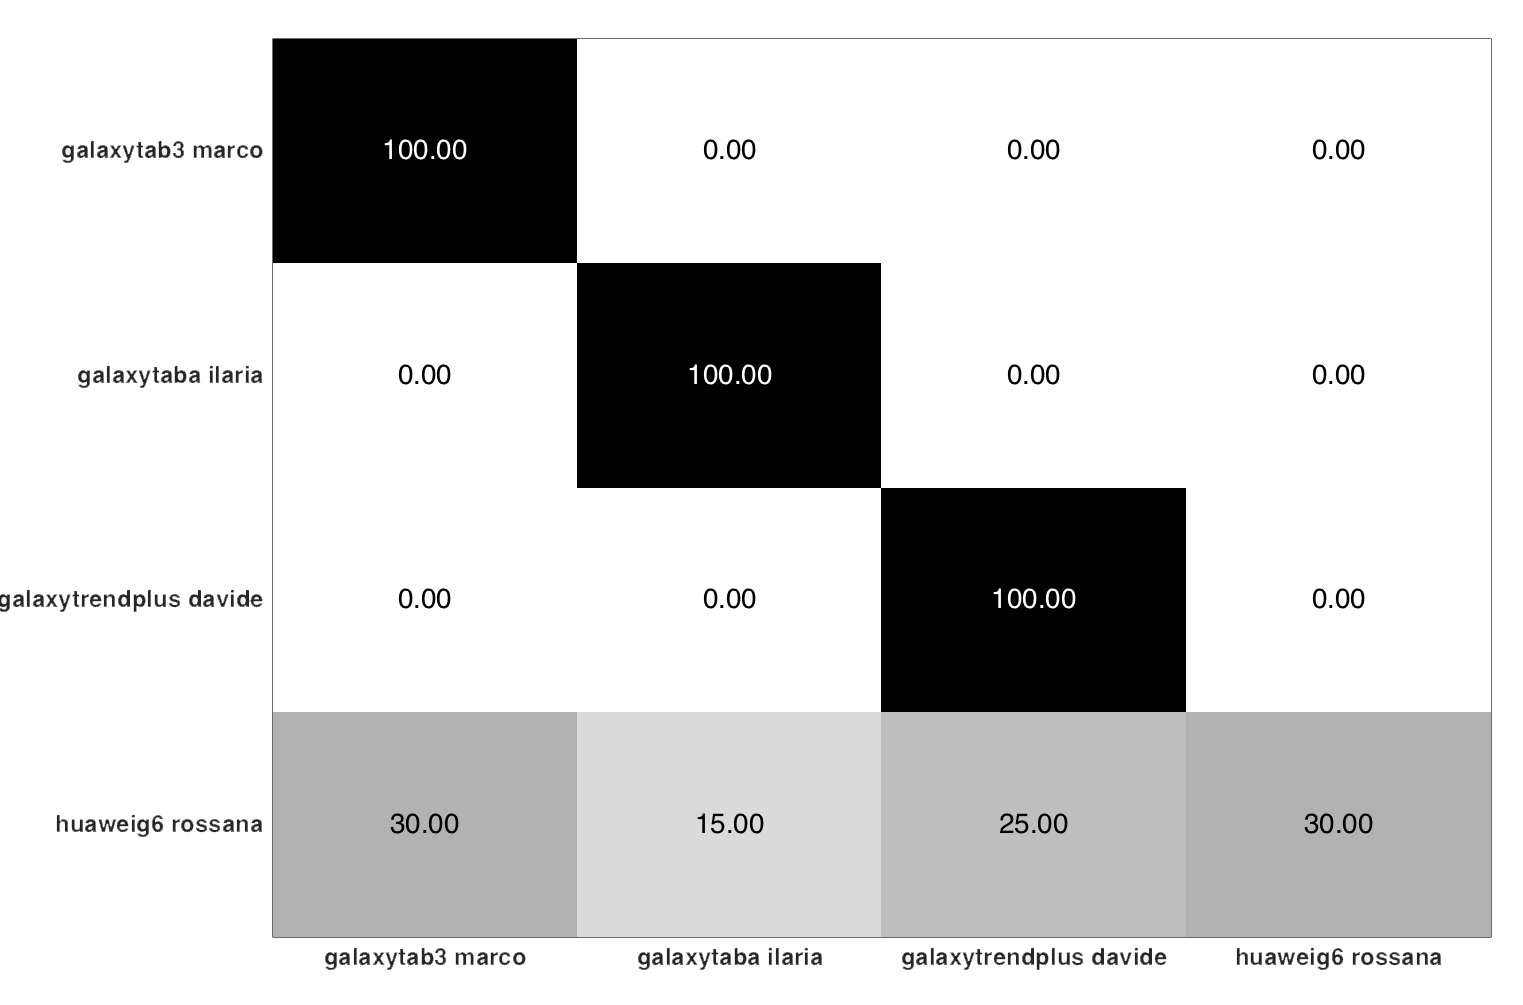
\includegraphics[width=0.4\textwidth]{images/confusionmatrix_nat_4.png}
\end{center}
  \caption{Matrice di confuzione per il caso delle immagini naturali usando 4 dispositivi.}
\label{fig:validation}
\end{figure}

\begin{figure}[h]
\begin{center}
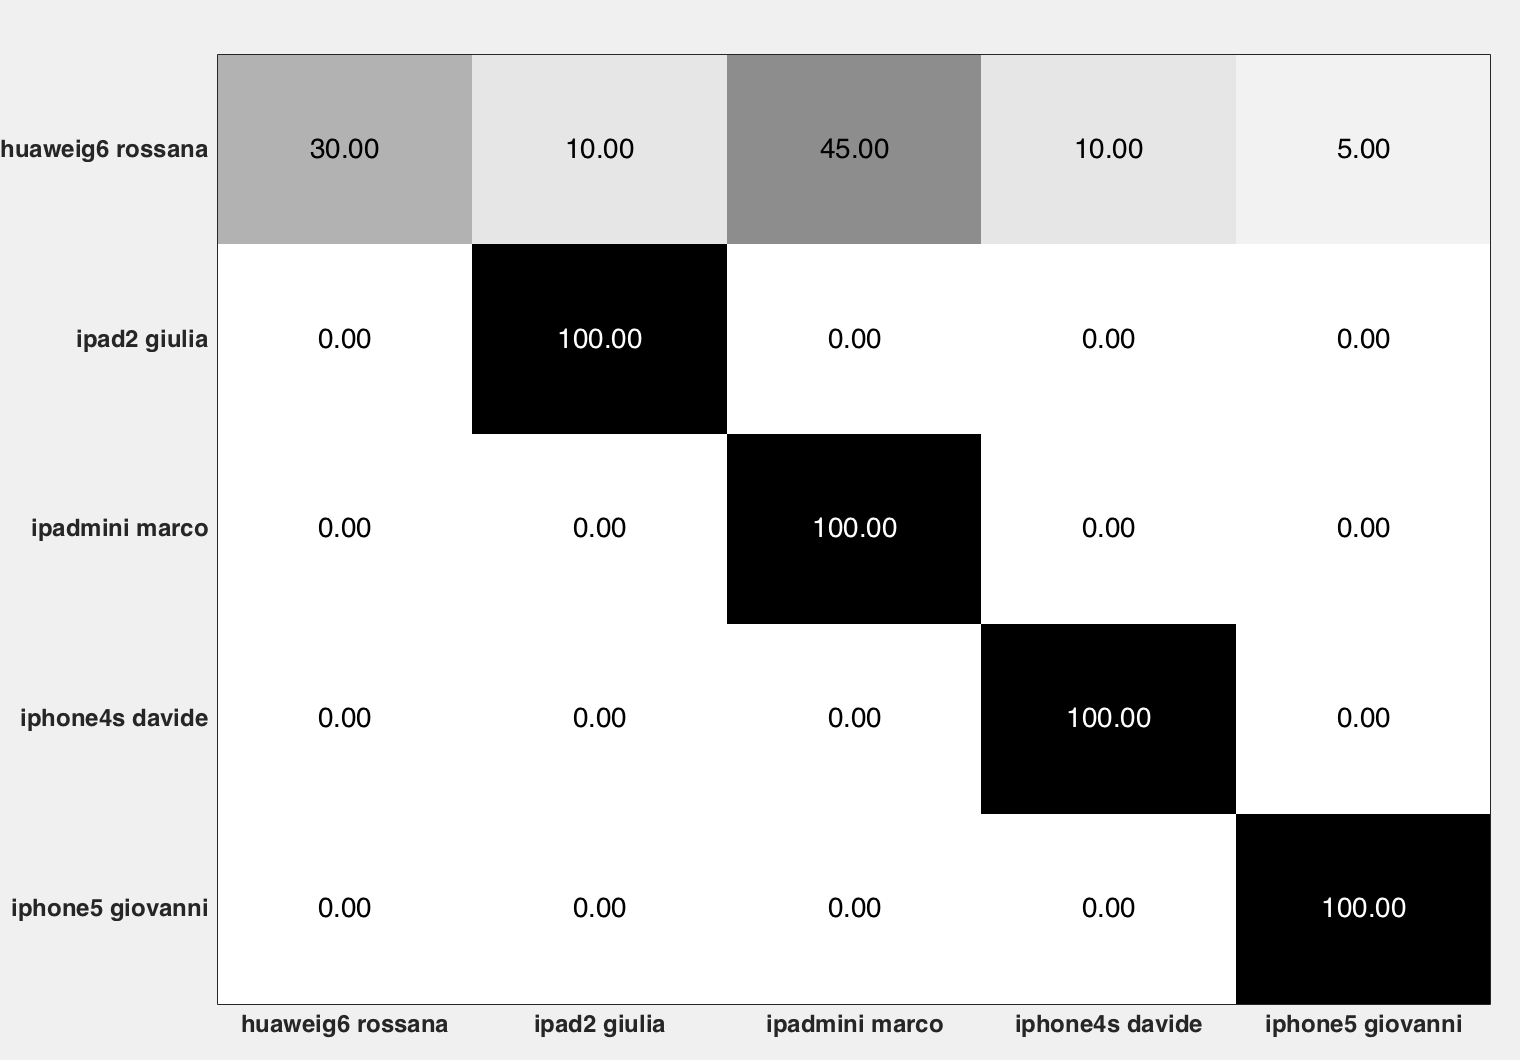
\includegraphics[width=0.4\textwidth]{images/confusionmatrix_nat_5.png}
\end{center}
  \caption{Matrice di confuzione per il caso delle immagini naturali usando 5 dispositivi.}
\label{fig:validation}
\end{figure}

\begin{figure}[h]
\begin{center}
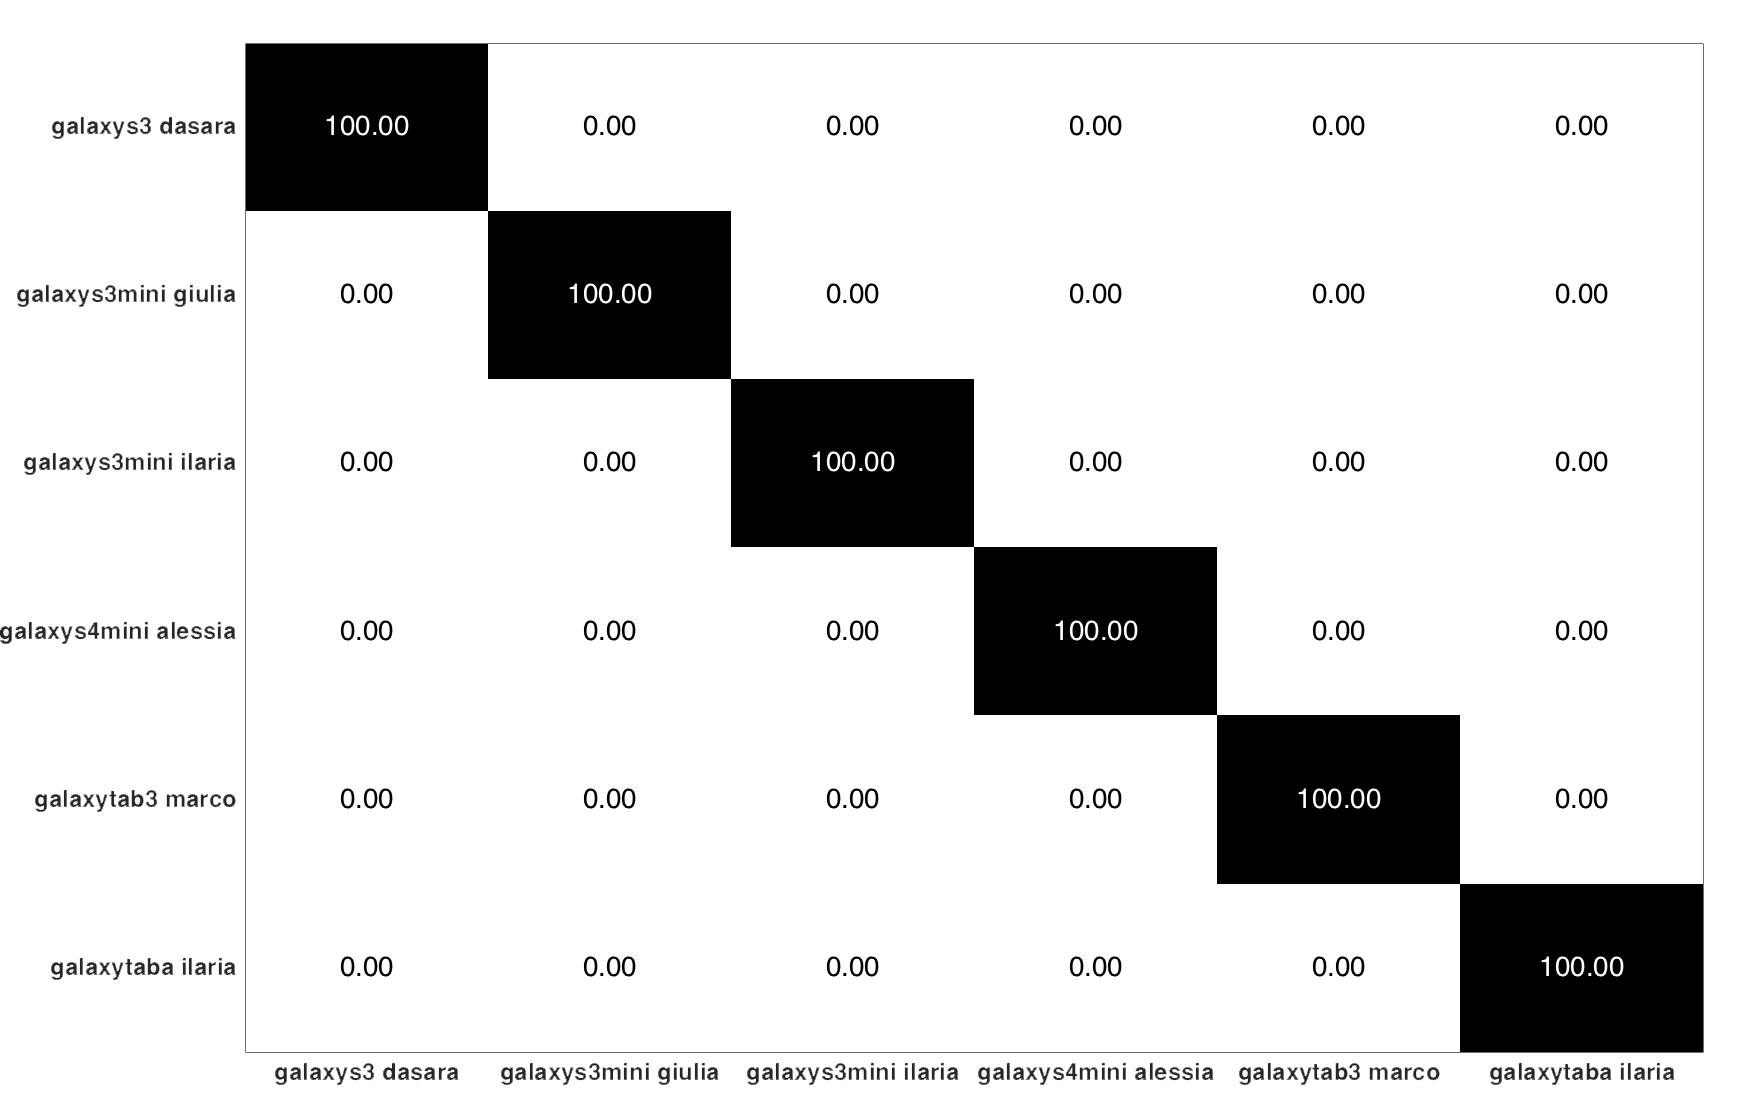
\includegraphics[width=0.4\textwidth]{images/confusionmatrix_nat_6.png}
\end{center}
  \caption{Matrice di confuzione per il caso delle immagini naturali usando 6 dispositivi.}
\label{fig:validation}
\end{figure}

Nel caso delle immagini naturali la validazione ottiene dei buoni risultati rispetto a tutte e tre le ripartizioni del dataset. Le immagini di validazione vengono associate alla giusta fingerprint con un'accuratezza del 100\% su tutti i dispositivi; l'unica eccezione è rappresentata dal dispositivo Huawei G6. Gli errori in questo caso non sono però dovuti ad una fingerprint rumorosa, poichè nella fase di clustering è stata ottenuta una percentuale di falsi positivi pari a 0. L'errore di classificazione è quindi dovuto in fase di validazione, ovvero quando, utilizzando la PCE viene calcolata la similitudine fra le immagini di test e le fingerprint estratte.

\begin{figure}[h]
\begin{center}
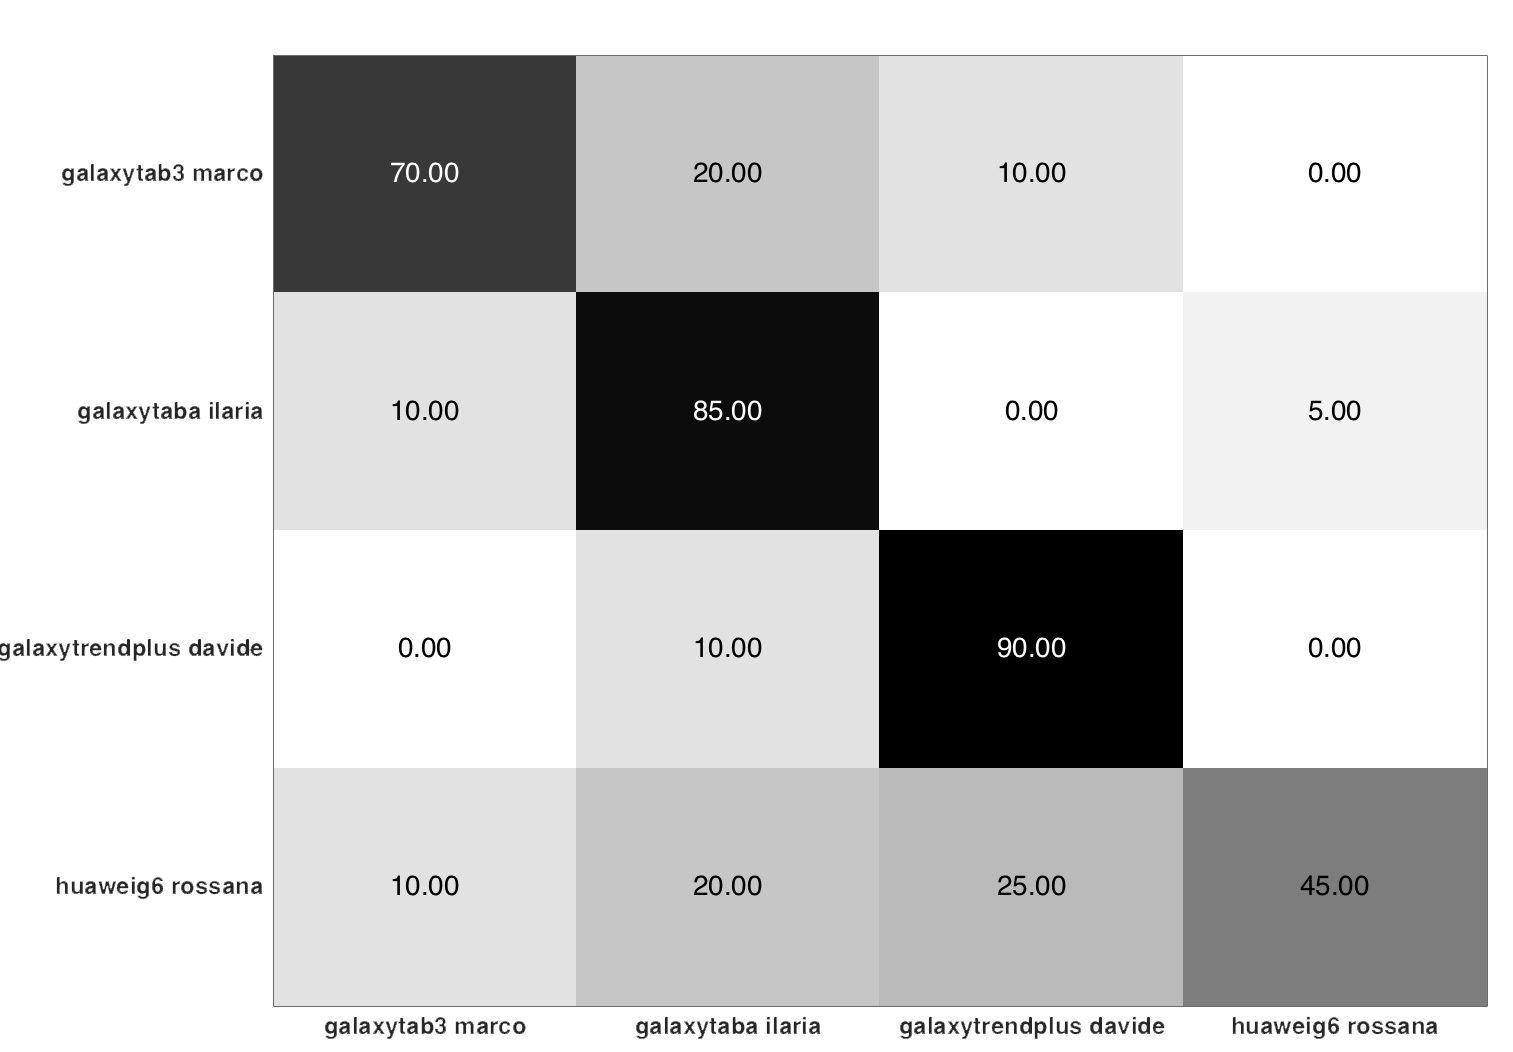
\includegraphics[width=0.4\textwidth]{images/confusionmatrix_fb_4.png}
\end{center}
  \caption{Matrice di confuzione per il caso delle immagini scaricati da Facebook usando 4 dispositivi.}
\label{fig:validation}
\end{figure}

\begin{figure}[h]
\begin{center}
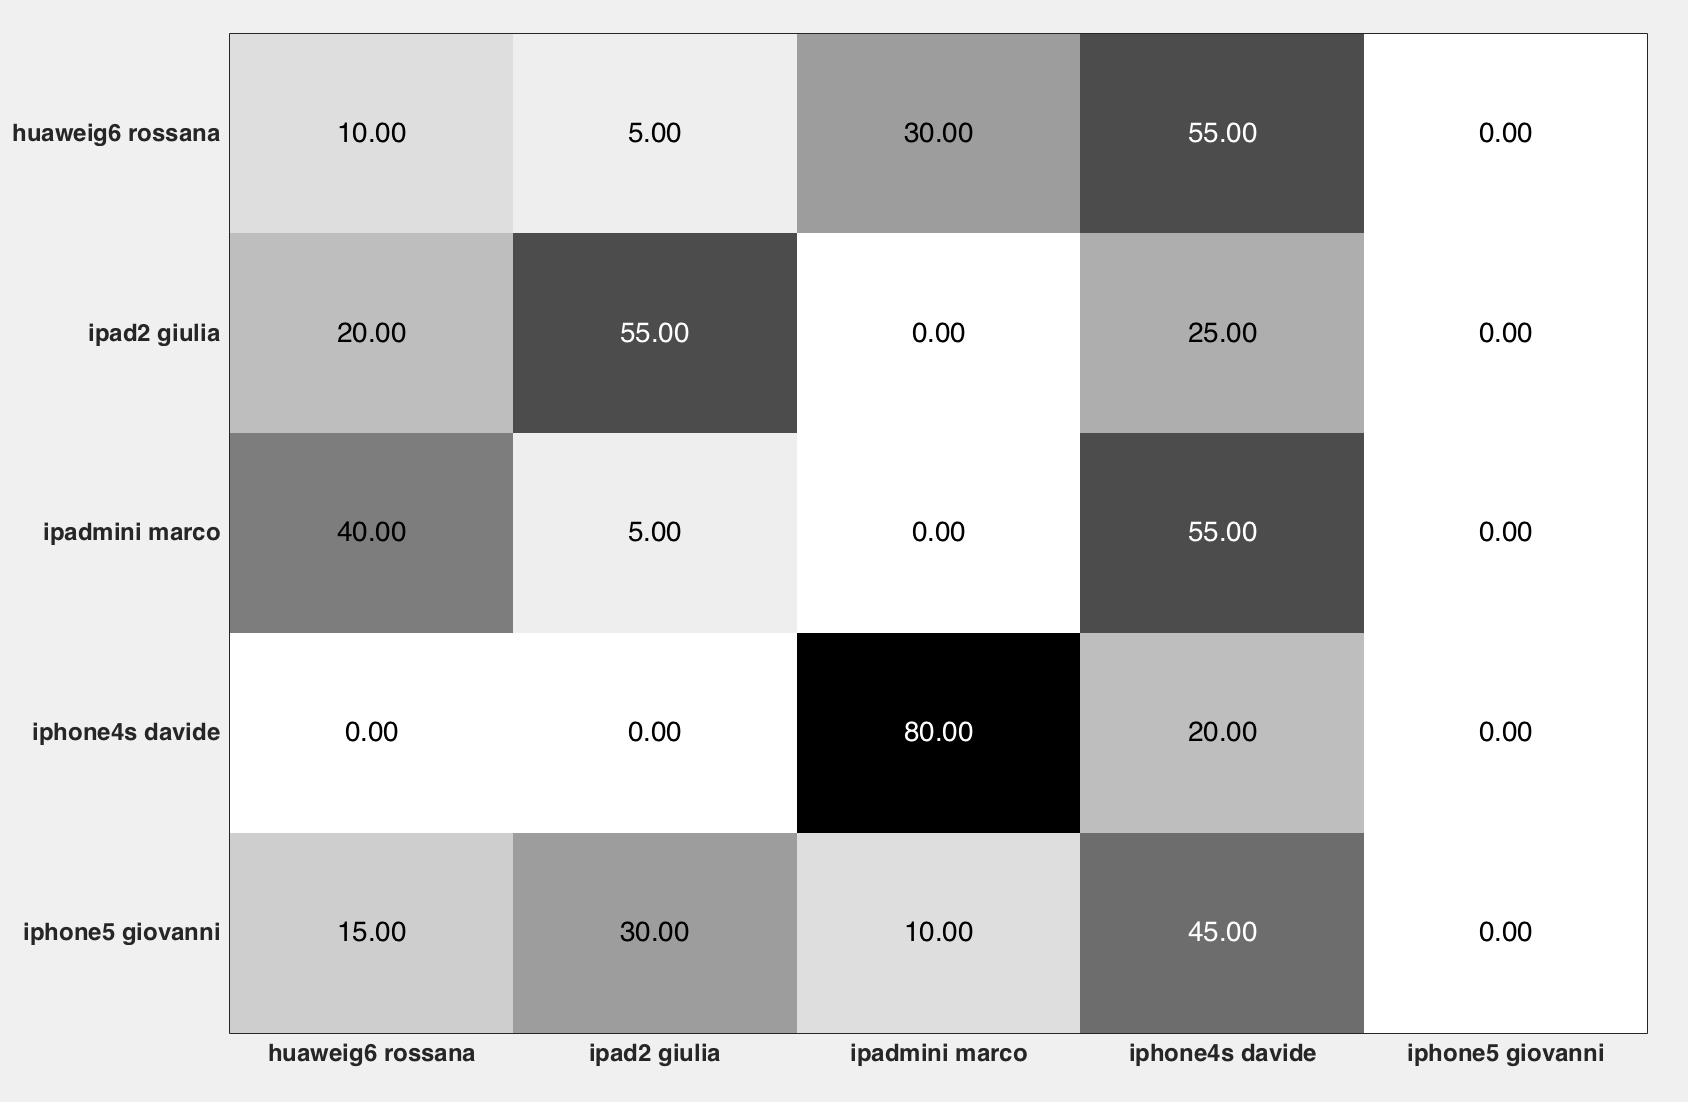
\includegraphics[width=0.4\textwidth]{images/confusionmatrix_fb_5.png}
\end{center}
  \caption{Matrice di confuzione per il caso delle immagini scaricati da Facebook usando 5 dispositivi.}
\label{fig:validation}
\end{figure}

\begin{figure}[h]
\begin{center}
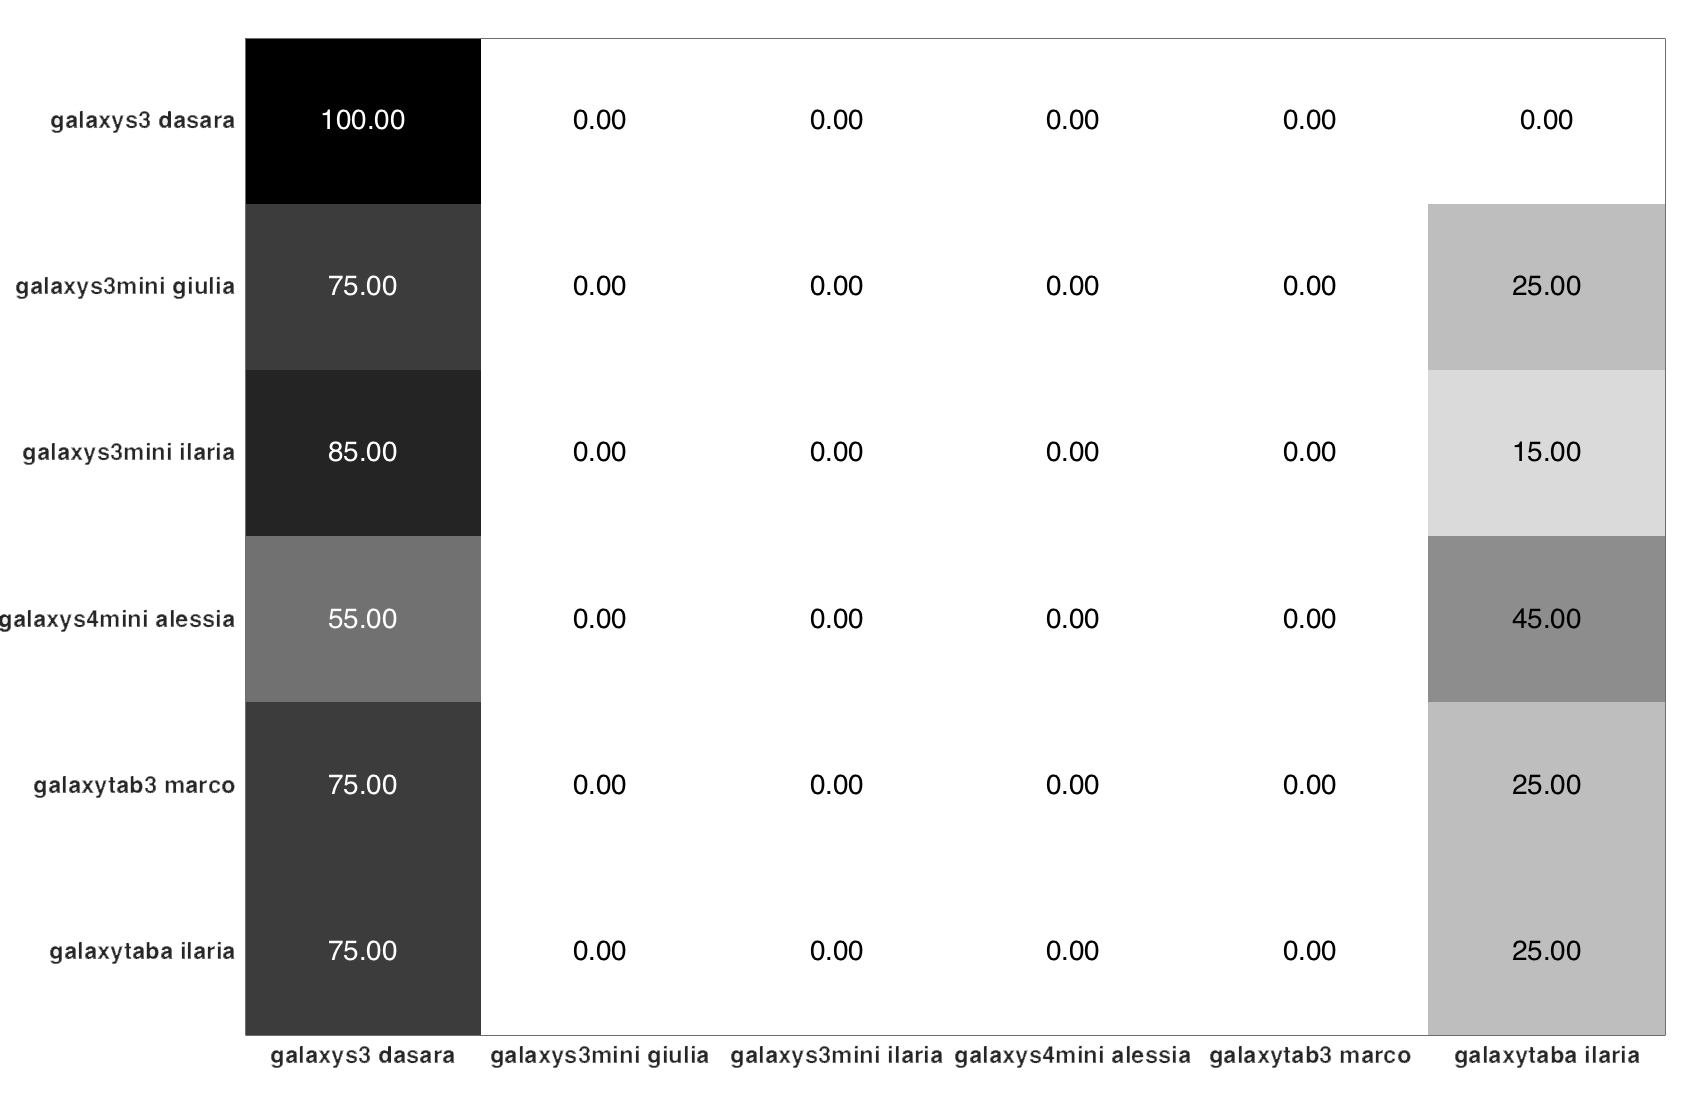
\includegraphics[width=0.4\textwidth]{images/confusionmatrix_fb_6.png}
\end{center}
  \caption{Matrice di confuzione per il caso delle immagini scaricati da Facebook usando 6 dispositivi.}
\label{fig:validation}
\end{figure}

Nel caso delle immagini scaricate da Facebook, i risultati sono molto differenti. Solamente l'insieme da 4 dispositivi, sempre ad eccezione del dispositivo Huawei G6, presenta valori accettabili. A differenza del precedente, in questo caso i molteplici errori di classificazione sono dovuti alla fase di clustering. Come mostrato nella sezione sulla selezione della soglia per il clustering, è difficile trovare una soglia che produca una clusterizzazione corretta e priva di falsi positivi, cosa che incide sulla qualità delle fingerprints. Inoltre, essendo tali immagini compresse rispetto a quelle naturali, queste perdono in informazione e così la PRNU estratta è meno significativa. Infatti i valori medi della matrice dei pesi, calcolati con la PCE,  in questo caso sono all'incirca di un ordine di grandezza inferiore rispetto ai valori medi della matrice dei pesi del caso delle immagini naturali. Ciò si ripercuote sulla soluzione dell'equazione che Normalized Cuts utilizza per partizionare il grafo.

Si può dedurre dai risultati che il nostro metodo di identificazione automatica dei dispositivi non è efficace per immagini che hanno subito una compressione, poichè le PNRU non sono sufficientemente discriminanti. Per quanto riguarda le immagini naturali, i risultati della validazione sono molto buoni ad eccezione di un unico dispositivo.